\section{Methods}
\subsection{Study area}
\label{subsec:studyA1rea}
The study system for this investigation is the Drink area, a 7056 ha area on the east slopes of the Cascade Mountain Range in the Deschutes National Forest (see Figure \ref{fig:drinkOverview}). The US Forest Service has identified three objectives for the area.

\begin{figure}[ht]
\centering
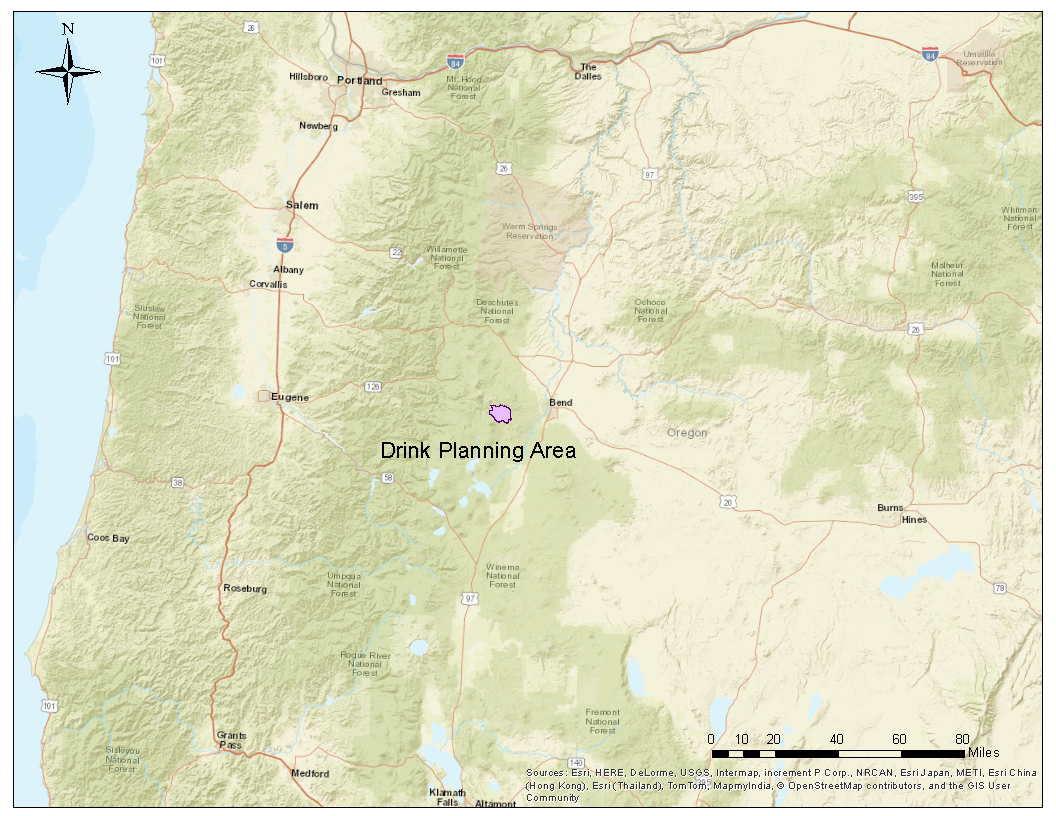
\includegraphics[width=.85\textwidth]{../images/DrinkMap_Overview}
\label{fig:drinkOverview}
\caption[Overview of the study system, the Drink Planning Area]{Overview of the study system, the Drink Planning Area (in dark purple), which is located in the Deschutes National Forest near Bend, Oregon.}
\end{figure}

\begin{figure}
\centering
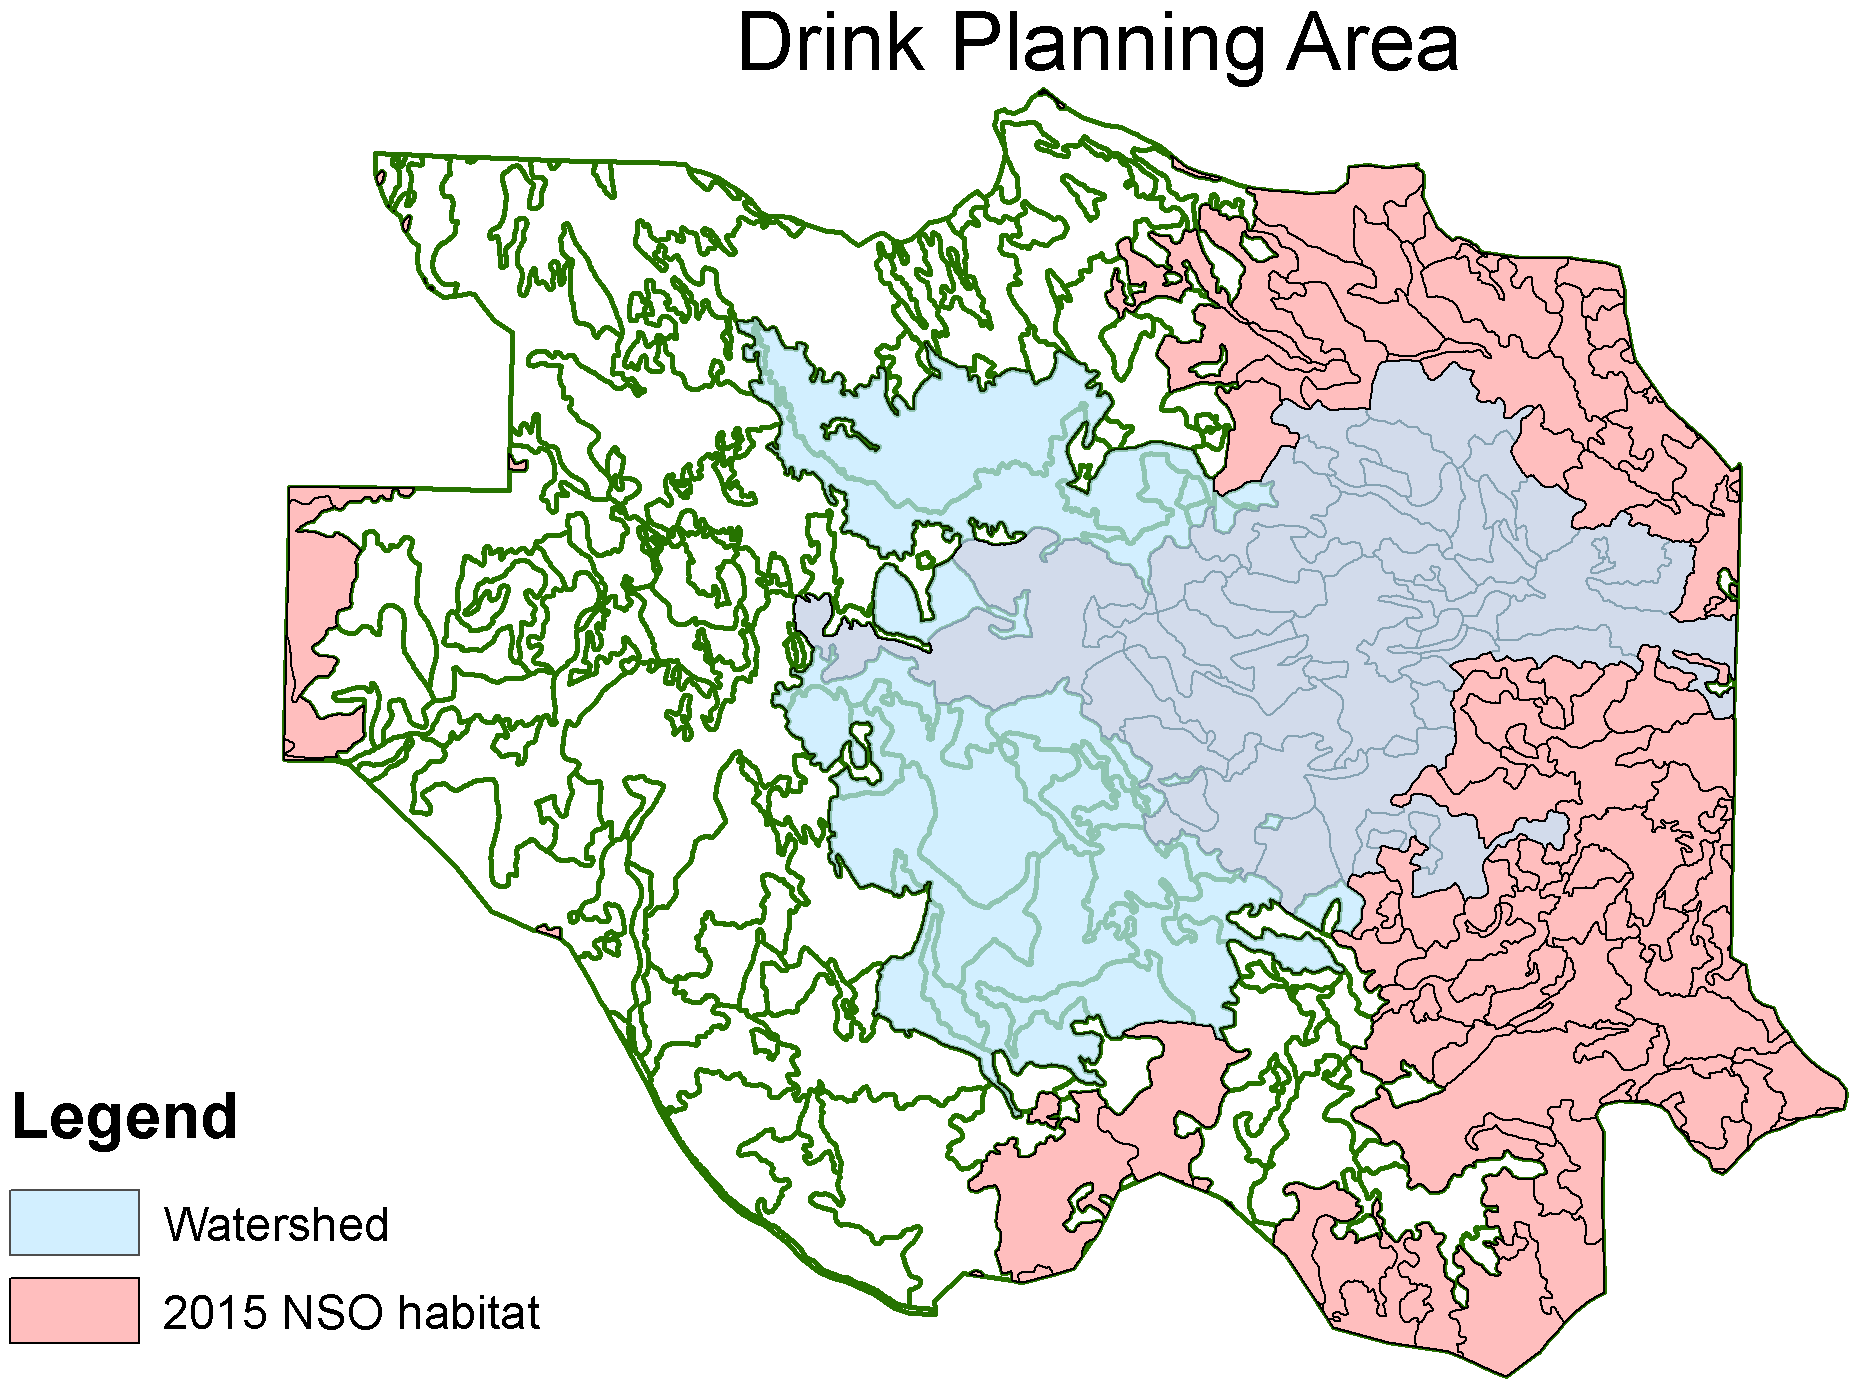
\includegraphics[width=.5\textwidth]{../images/DrinkMap_NSOAndWatershed}
\label{fig:drinkOwlAndWatershed}
\caption[NSO Habitat and municipal watershed in the Drink Area]{Location of the municipal watershed and the suitable NSO habitat in the Drink area at the beginning of the planning horizon (2015). Interior polygons are the 303 management stands.}
\end{figure}

The first objective is the reduction of fire hazard through the use of silvicultural treatments. This objective was chosen because one third of the Drink area comprises the municipal watershed for the cities of Bend, OR and Sisters, OR (see Figure \ref{fig:drinkOwlAndWatershed}) which have a combined population of approximately 90,000. Wildfires pose a threat to the watershed as they cause soil water repellency, surface runoff, and debris torrents \cite{ice2004effects}. In addition, approximately 60\% of the Drink serves as habitat for the northern spotted owl (NSO) (\textit{Strix occidentalis caurina}). While controversy exists over the NSO's status as an indicator or umbrella species \cite{simberloff1998flagships}, the USFS is nonetheless required to protect it since the NSO is threatened and therefore covered by the Endangered Species Act of 1973 \cite{congress1973endangered}. The protection of NSO habitat is the second objective I consider in this analysis. Lastly, I consider the minimization of the sediment delivered to the watershed as a result of the treatments applied to reduce fire hazard. While the treatments aim to provide long-term protection of the watershed's quality, they also have the potential to introduce short-term increases in sediment delivery \cite{o2005conceptual}.

\begin{figure}
\centering
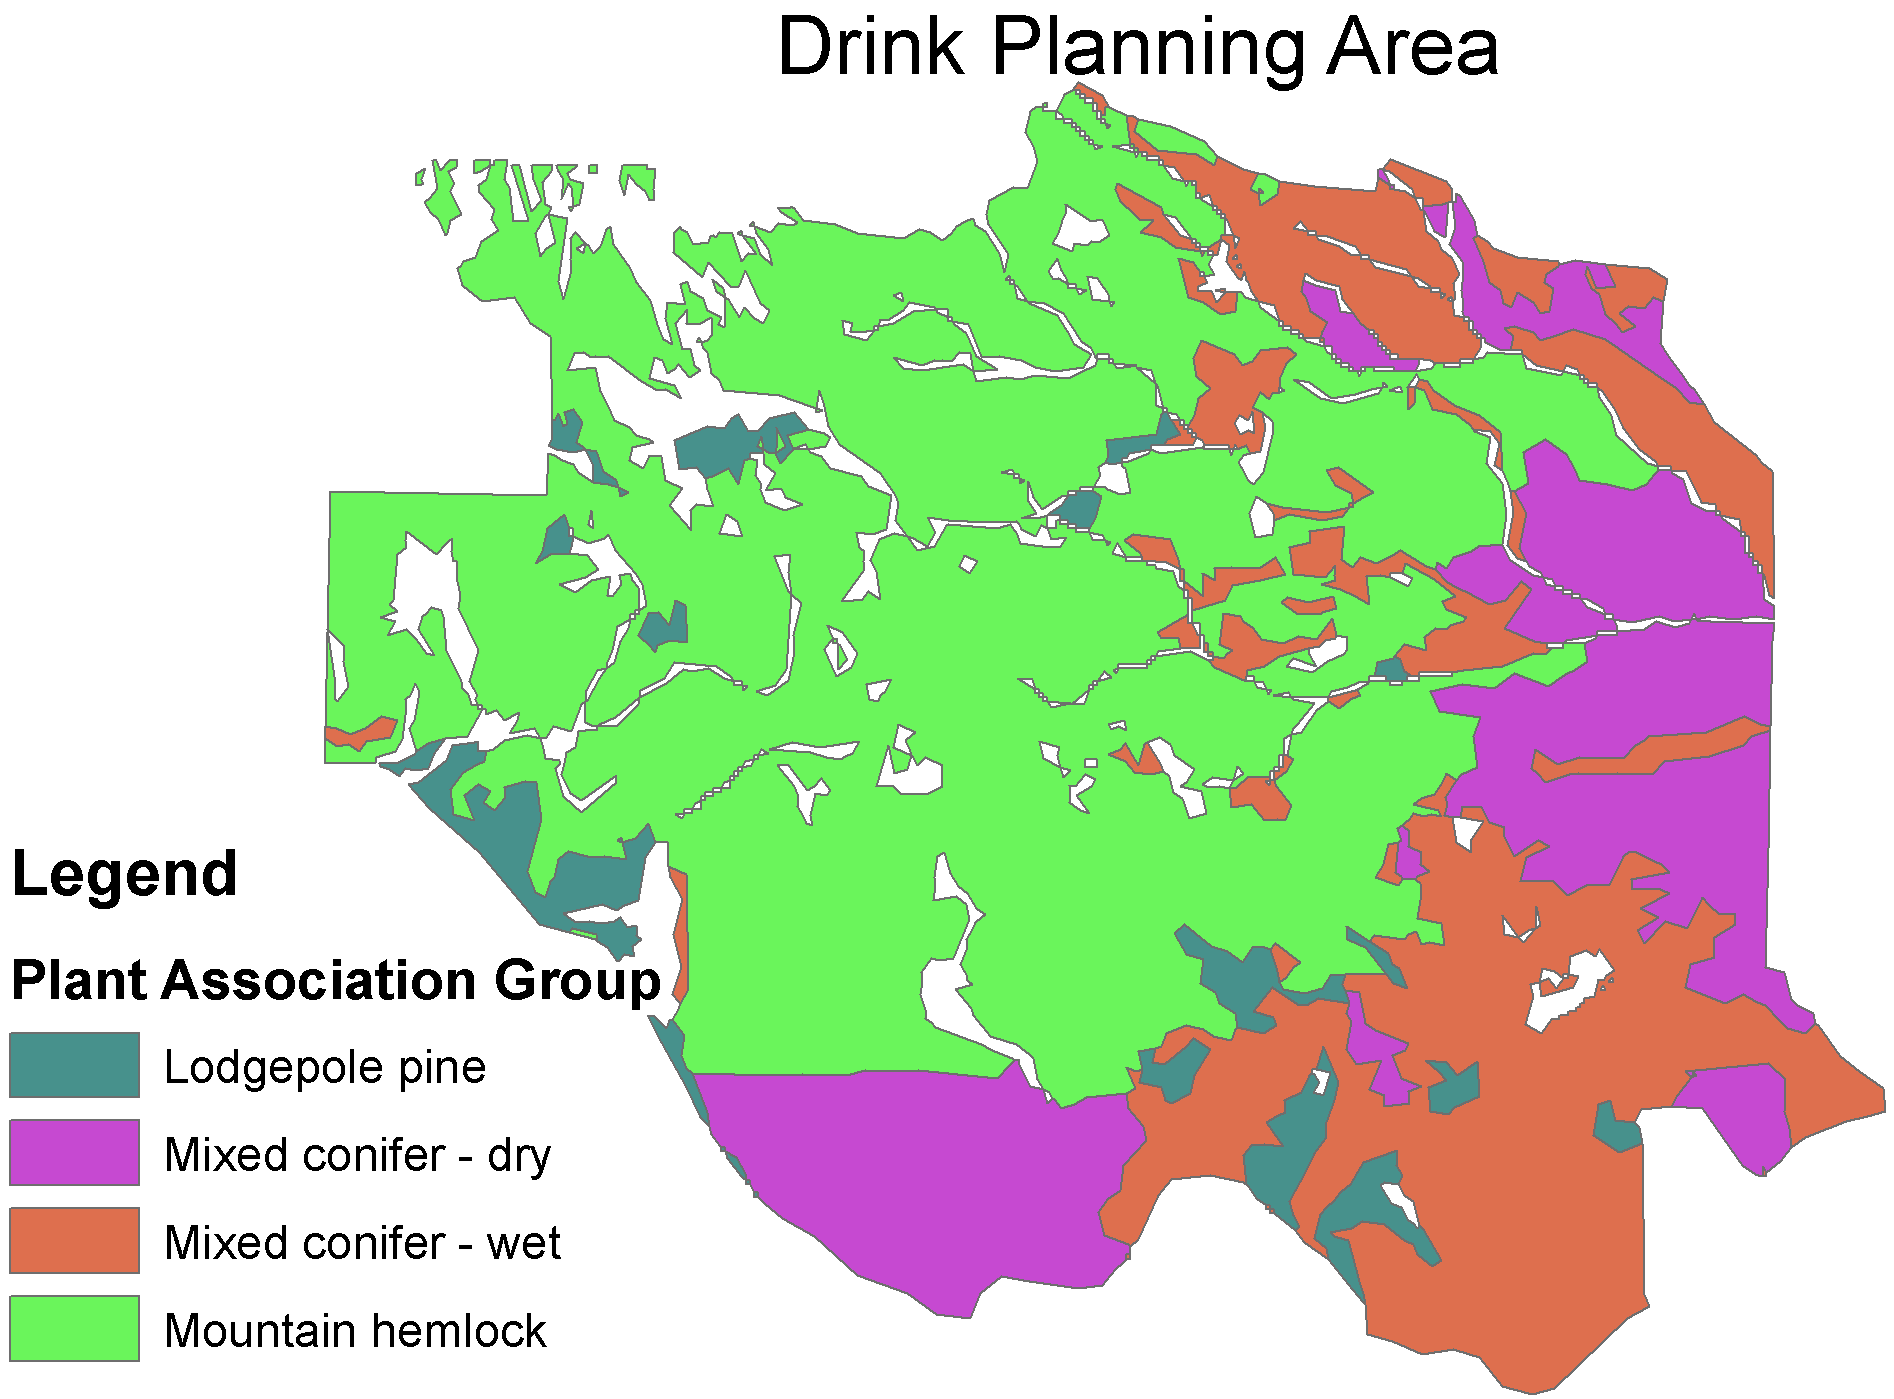
\includegraphics[width=.5\textwidth]{../images/DrinkMap_PAGs}
\label{fig:drinkPAGs}
\caption[Plant association groups in the Drink Planning Area]{Plant association groups in the Drink Planning Area selected for treatment by the US Forest Service.}
\end{figure}

To accomplish the long-term reduction in fire hazard, I will form a strategic plan for silvicultural treatments to apply across the Drink area. The treatments may be applied in each of two 20-year time periods (2015-2035 and 2035-2055) and to each of the 303 management units that comprise the Drink. The division of the management units (stands) was performed \textit{a priori} by the Forest Service. The decision as to which treatment to perform on a stand is entirely dependent on silvicultural characteristics; the specifications can be found in Appendix \ref{chap:appBTreatmentSpec}. To assess the treatments' long-term efficacy, I measure the fire hazard of the Drink at the end of an 80-year planning horizon (2015-2095). I also measure the area of NSO habitat at the end of the 80-year planning horizon. The short-term sediment contributions from performing the treatments are measured at the time of treatment, which is assumed to be at the midpoint year in the planning period (either 2025 for period 1 or 2045 for period 2). The time of these events in the planning horizon is shown in Figure \ref{fig:drinkPlanningHorizon}.
\begin{figure}
\centering
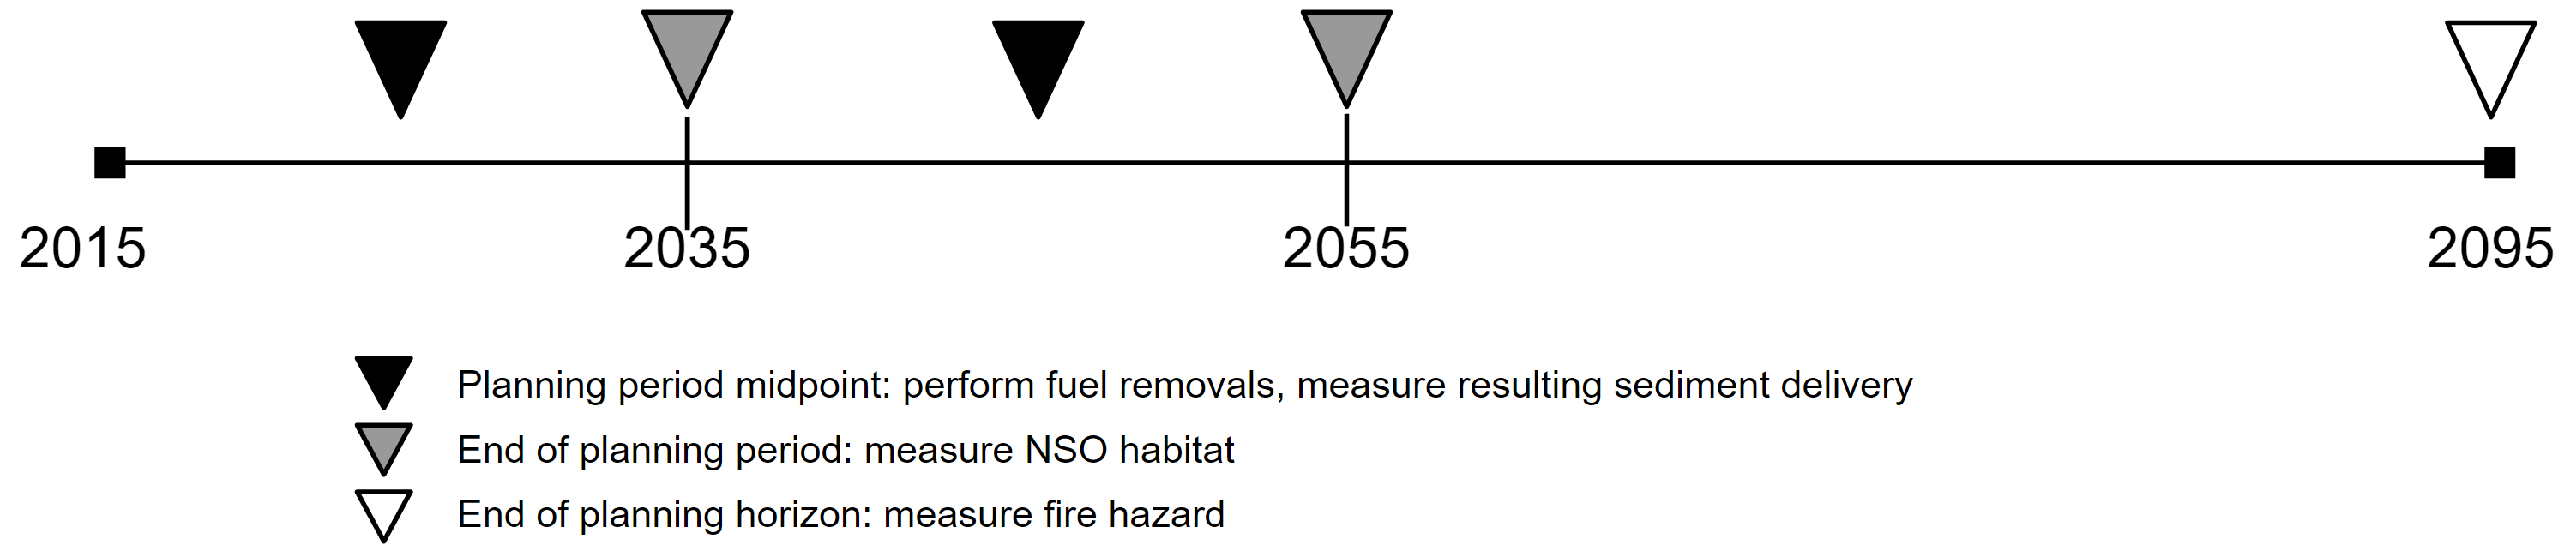
\includegraphics[width=.75\textwidth]{../images/Drink_PlanningHorizon_Sketch}
\label{fig:drinkPlanningHorizon}
\caption[Planning horizon schematic]{The planning horizon used in the analysis spans the 80 year period from 2015 to 2095. Treatments may be performed in the first period (point 1), second period (point 2), both, or neither. Treatments are assumed to be performed at the mid-point years of each period (points 1 and 2). Sediment delivery is measured on treatment years. I assess the stands' suitability for NSO habitat and their fire hazard at the end of the planning horizon (point 3).}
\end{figure}

Notice that the three objectives are inherently in conflict with one another: fuel treatments drive short-term sediment delivery and the potential reduction of owl habitat; minimizing short-term sediment delivery entails fewer treatments and a higher fire hazard; maximizing owl habitat may require forgoing fuel treatments and again lead to higher fire hazard. In this study, I will determine how climate change impacts the tradeoffs that exist among these objectives.

\subsection{Choosing Climate Scenarios for Comparison}
To determine the impacts of climate change on the tradeoff structure between ecosystem services, it is first necessary to define how the impacts of climate change are to be captured in the analysis. I do this in the current study using the method employed by the IPCC, namely, through a scenario-based analysis. In a scenario analysis, multiple alternative futures are considered and no prediction is made as to which scenarios are more likely than others. There is no attempt to quantify the probability of realization of any one scenario.

The alternative futures I consider here are climate scenarios. Given the large number of potential future climates considered by the IPCC (see \cite{ipccListOfAR5Models}) combined with the computational complexity involved in the study of each one, I selected a small subset of  future climate scenarios for my analysis. These are ``None'', ``Ensemble RCP 4.5'', and ``Ensemble RCP 8.5''.

The first scenario, ``None'', is the assumption of no climate change. While the number of studies incorporating climate change is increasing, this is still the assumption used for many modern studies such as \cite{svetlanaDissertation2013}, from which this study is derived. Because it has served as the basis for many studies and assumes a static environment resembling today's, the ``None'' climate scenario is the control against which I compare the other two climate scenarios.

As their names suggest, the second and third scenarios are ensembles of future climate projections. The components of the ensembles are global circulation models (GCMs) used in the IPCC's Fifth Assessment (AR5). The USFS's Climate-FVS \cite{dixon2002essential} team selected the ensemble components and created the climate surface corresponding to the collection of these 17 GCMs. The list of the 17 scenarios included in the ensemble can be found in \cite{ClimateModelsInFVSEnsemble}. The climate surface contains a vector of 35 climate parameters at over 11,000 global locations for three time periods \cite{crookston2014climate}. This provides a climate surface for each of the scenarios that, while temporally sparse, is spatially robust. This configuration is useful for the Drink area given its variability in elevation and slow growth.

The ensembles differ in the representative concentration pathway (RCP) assumed in the comoponent GCMs. The RCP indicates the additional radiative forcing (in $W/m^2$) above pre-industrial levels, with higher values of forcing indicative of more severe climate change. The GCMs in Ensemble RCP 4.5 assume 4.5 $W/m^2$ of additional radiative forcing, and the GCMs in Ensemble RCP 8.5 assume 8.5 $W/m^2$ of additional radiative forcing.

I chose these three scenarios because they represent a range of predicted severity of climate change, from a $0 \degree C$ warming by the year 2100 under the ``None'' scenario to a $2.6-4.8 \degree C$ warming under RCP 8.5 \cite{ipcc2013climate}.

\subsection{Generating tradeoff relationships between ecosystem services}
\label{subsec:whyUsingMultiObjModel}
With this selection of climate scenarios, how can one determine the relationships between ecosystem services under each scenario? One applicable method is multi-objective mathematical optimization \cite{TothFsci2009}. This approach seeks to maximize a set of objectives subject to a set of constraints. I define my objectives as the ecosystem services that the USFS prioritized for the Drink area (\S \ref{subsec:studyArea}). The set of constraints was determined through a combination of input from the USFS and logical constraints. The latter includes restrictions such as that one may not perform silvicultural treatments to areas that are not forested; the former includes such restrictions as how many acres may be treated in a given year.

The multi-objective model, or mathematical program, that I built and used for this analysis is described below. The program involves linear, integer, and binary variables, making it a mixed integer program (MIP). The treatment assignment rules for the model, the acquisition of the required data, and the projection of that data into the future are described here:

\subsubsection{Treatment scheduling and assignment rules}
I simulated the 303 stands in the Drink area over the course of an 80 year planning horizon with all treatment activity occurring in the first 40 years. The activity could be selected to be completed in the first twenty year period, the second twenty year period, both, or neither. The type of treatment to be performed is dependent on silvicultural characteristics (see \S \ref{chap:appBTreatmentSpec}) and was determined \textit{a priori} using the vegetation data described below. As a result, the model needed only to choose whether to perform a treatment on a stand in a given period; the model did not have to select which treatment to perform.

\subsubsection{Acquisition and projection of data}
The data required to solve the model include - for each climate scenario, each time period and each stand - a measure of fire hazard, determination of suitability for NSO habitat, and the amount of sediment deposited in the municipal watershed as a result of performing various thinning treatments.

As a measure for fire hazard, I chose the average fuel model of a stand according to the Anderson fuel model rating system \cite{anderson1982aids}. This fuel model rating is an integer 1-13, that describes the fuel characteristics of an area, with larger fuel models corresponding to larger fuel loads, making it a suitable proxy for fire hazard. To determine the initial fuel models of each stand, I obtained the 2012 GNN structure map (\url{http://lemma.forestry.oregonstate.edu/data/structure-maps}) from Oregon State University's Landscape Ecology, Modeling, Mapping \& Analysis (LEMMA) group. The LEMMA group provides this data in a format compatible with the USFS's Forest Vegetation Simulator (FVS). I used FVS's database extension to import this data into FVS and then used FVS's Fire and Fuels Extension\cite{reinhardt2003fire} (FFE) to compute the average fuel model for each stand. I then used Climate-FVS to project the stands' vegetation forward 80 years until the end of the planning horizon under each of the climate scenarios.

Through previous conversations with the USFS, it was determined that any area meeting the following characteristics would be considered ideal NSO habitat:
\begin{enumerate}
\item elevation less than 1830 m
\item the presence of trees with DBH no less than 76 cm
\item canopy closure of at least 60\%
\item greater than 200 ha in size
\end{enumerate}
I attained a digital elevation model from the US Department of Agriculture's GeoSpatial Data Gateway to compute average stand elevation and check for the first criterion. I checked the second and third criteria using the vegetation data produced by FVS. If the first three criteria are met but the area is not 200 ha in size, it is still classified as NSO habitat but is penalized by a factor of $e = 0.5$. Since stands were generally less than 200 ha in size, the last criterion required the enumeration of all clusters of stands whose combined contiguous area exceeded 200 ha. The model checks whether all stands in such a cluster meet the first three criteria to determine whether the penalization is required.

I retrieved data on sediment delivery using the Watershed Erosion Prediction Project (WEPP) online GIS tool \cite{frankenberger2011development}. This tool takes as input soil textures, treatment types, years of simulation, and custom climate data. I obtained soil texture data for the area from the USDA's Soil Survey Geographic (SSURGO) database. Treatment types are those specified in \S \ref{chap:appBTreatmentSpec}, and the years of simulation correspond to the planning horizon of the model. The custom climate data was obtained through the Climate-FVS climate data server \cite{climateFVSReadyData}. Using the climate data provided by Climate-FVS in the sediment delivery simulations ensured consistency of climate parameters with the simulations for the Drink's vegetation.

\subsubsection{The Multi-objective MIP}
The first objective in the model is to minimize the average fuel model at the end of the 80-year planning horizon:
\begin{align}
Minimize \quad & F = \sum_{i\in I} \sum_{r\in R} F_{i,r} x_{i,r} \label{eqn:objFire}
\end{align}
In equation \eqref{eqn:objFire}, I sum over all stands $i \in I$ and all treatment prescriptions $r \in R$ to obtain a cumulative fire hazard metric $F$, which measures the total fire hazard of the area at the end of the planning horizon. The coefficients $F_{i,r}$ are the area-weighted fuel models of each stand $i \in I$ at the end of the planning horizon if stand $i$ is assigned to treatment prescription $r \in R$. The possible treatment prescriptions $r \in R$ are treat in the first period ($r=1$), treat in the second period ($r=2$), treat in both periods ($r=3$), or do not treat ($r=0$).

The second objective is to minimize the peak short-term sediment delivery that results from performing treatments in either period one ($S_1$) or period two ($S_2$):
\begin{align}
Minimize \quad S = \max \{S_1,S_2\} \label{eqn:objSediment}
\end{align}

The last objective is to maximize the area of suitable northern spotted owl habitat at the end of the planning horizon.
\begin{align}
Maximize \quad & O = \sum_{i\in I_\omega} \left(a_i p_i + e a_i \left( \sum_{j \in R_i} x_{i,j}-p_i \right) \right) \label{eqn:objOwl}
\end{align}
The set of stands in the sum $i \in I_\omega$ are those that meet the first three criteria for NSO habitat under at least one treatment prescription $j \in R_i$, where $R_i$ is the set of treatment prescriptions for stand $i$ such that it meets the first three NSO habitat criteria at the end of the planning horizon. If a stand $i$ does not meet these criteria under any treatment prescriptions (if the set $R_i = \{\emptyset\}$), then $i \notin I_\omega$. If the model assigns a stand $i \in I_\omega$ a treatment prescription $j \in R_i$, then stand $i$ meets the first three NSO habitat criteria at the end of the planning horizon, and the variable $x_{i,j}=1$. If, in addition, the stand $i$ is part of a cluster of stands all meeting the first three NSO habitat criteria and whose combined contiguous area is greater than 200 ha, then the variable $p_i = 1$. Notice that when $p_i = 0$, the stand's contribution is discounted by $e = 0.5$, and when $p_i = 1$ it is not.

The objectives are subject to the following constraints. First, I define accounting variables for the sediment delivery that results from the performance of the prescribed management actions.
\begin{align}
\sum_{i\in I} \sum_{r\in 1,3} s_{i,1} x_{i,r} = S_1 \label{eqn:constraintSediment1}\\
\sum_{i\in I} \sum_{r\in 2,3} s_{i,2} x_{i,r} = S_2 \label{eqn:constraintSediment2}
\end{align}
The coefficients $s_{i,t}$ are the amount of sediment (in tonnes) that would result from treating stand $i$ in time period $t$.

In order to control the trigger variables $p_i$ indicating a stand's inclusion in a 200 ha cluster of NSO habitat, I used the following two constraints:
\begin{align}
\sum_{i \in D_c} \sum_{j \in R_i} x_{i,j} - |c| q_c &\ge 0 \qquad \forall c \in C \label{eqn:constraintClusterTriggers}\\
\sum_{c \in C_i} q_c - p_i &\ge 0 \qquad \forall i \in I_\omega \label{eqn:constraintPVarTriggers}
\end{align}
$c \in C$ are the clusters of stands whose combined area is greater than 200 ha. A cluster $c$ contains the set of stands $i \in D_c$. Equation \eqref{eqn:constraintClusterTriggers} specifies that all stands $i \in D_c$ within a cluster $c \in C$ must be assigned a management prescription such that they meet all NSO habitat criteria in order for the cluster trigger variable $q_c$ to take value 1.

Equation \eqref{eqn:constraintPVarTriggers} specifies that if no cluster $c \in C_i$ - the set of clusters that contain site $i$ - meets NSO qualifications, then the trigger variable $p_i$ must equal 0. If some cluster $c \in C_i$ does meet NSO qualifications, then the objective function \eqref{eqn:objOwl} will draw up the value of the variable $p_i$ to 1.

I also impose the restriction that each stand may be assigned to at most one treatment prescription.
\begin{align}
\sum_{r \in R} x_{i,r} = 1  \qquad \forall i \in I \label{eqn:constraintOnePrescrip}
\end{align}

Next, I ensured that the area treated in each time period is less than a prespecified maximum area $A$:
\begin{align}
\sum_{i \in I} \sum_{r \in 1,3} a_i x_{i,r} &= H_1 \label{eqn:constraintAreaAcctg1}\\
\sum_{i \in I} \sum_{r \in 2,3} a_i x_{i,r} &= H_2 \label{eqn:constraintAreaAcctg2}\\
H_1 &\le A \label{eqn:constraintAreaRestr1}\\
H_2 &\le A \label{eqn:constraintAreaRestr2}
\end{align}
where the first two equations define the accounting variables for the areas treated in time periods 1 and 2, $H_1$ and $H_2$, and the second two equations impose the upper bound.

Finally, I specified fluctuation constraints to bound the differences in the area treated in between time periods:
\begin{align}
\ell H_1 - H_2 &\le 0 \label{eqn:constraintAreaFlucL}\\
-u H_1 + H_2 &\le 0 \label{eqn:constraintAreaFlucU}
\end{align}
I define a maximum of 20\% fluctuation between time periods. That is, $\ell = 0.8$ and $u = 1.2$.

Together with the binary specifications on our variables (equation \eqref{eqn:constraintNonNeg}), the complete model is
\begin{align*}
Minimize \quad & \\
F=&\sum_{i\in I}\sum_{r\in R} F_{i,r} x_{i,r}\\
S=&\max \{S_1,S_2\}\\
Maximize \quad & \\
O=&\sum_{i\in I_\omega} \left(a_i p_i + e a_i \left( \sum_{j \in R_i} x_{i,j}-p_i \right) \right)
\end{align*}

Subject to:
\begin{align}
\sum_{i\in I} \sum_{r\in 1,3} s_{i,r} x_{i,r} &= S_1 \notag\\
\sum_{i\in I} \sum_{r\in 2,3} s_{i,r} x_{i,r} &= S_2 \notag\\
\sum_{i \in D_c} \sum_{j \in R_i}x_{i,j} - |c| q_c &\ge 0 \qquad \forall c \in C \notag\\
\sum_{c \in C_i} q_c - p_i &\ge 0 \qquad \forall i \in I_\omega \notag\\
\sum_{r \in R} x_{i,r} &= 1  \qquad \forall i \in I \notag\\
\sum_{i \in I} \sum_{r \in 1,3} a_i x_{i,r} &= H_1 \notag\\
\sum_{i \in I} \sum_{r \in 2,3} a_i x_{i,r} &= H_2 \notag\\
H_1 &\le A \notag\\
H_2 &\le A \notag\\
\ell H_1 - H_2 &\le 0 \notag\\
-u H_1 + H_2 &\le 0 \notag\\
x_{i,r}, p_i, q_c \in \{0,1\} \quad &\forall i \in I, r \in R, c \in C \label{eqn:constraintNonNeg}
\end{align}

\subsection{Model solution}
Solving a bounded and non-degenerate multi-objective optimization problem with $N$ objectives produces a set of objective vectors (also called ``solutions'') $\mathbf{z} \in Z$ where $\mathbf{z}=\braket{z^1,\ldots,z^N}$. The set of solutions $Z$ is referred to as the Pareto-optimal frontier or efficient frontier or, simply, frontier. The solutions comprising an efficient frontier have the special relationship such that no component of a solution $\mathbf{z}^i$ can be improved upon without one of the other components $\mathbf{z}^j$ ($j \neq i$) degrading. For example, this relationship in the current problem means that further reducing fire hazard would require either additional sediment deposits, the sacrifice of NSO habitat, or both.

Thus the efficient frontier provides information on the tradeoff structure that exists between ecosystem services. Parameterizing and solving the model for each of the climate scenarios generates three frontiers: $Z_{\text{None}}$, $Z_{4.5}$, and $Z_{8.5}$ for the No climate change, Ensemble RCP 4.5, and Ensemble RCP 8.5 scenarios, respectively. As climate is the driver of the differences in these frontiers, the comparison of frontiers provides insight into how climate impacts the tradeoff structures between the ecosystem services.

To solve the models, I wrote my own implementation of T\'{o}th's Alpha-Delta algorithm \cite{TothThesis} that is generalized for any multi-objective problem with $N \ge 2$ objectives. The Alpha-Delta algorithm finds the optimal set $Z$ by iteratively slicing the $N$-dimensional objective space with a tilted $N-1$ dimensional plane. To derive the frontiers, I used an alpha parameter of $\alpha = .01$ and delta parameters of $\delta_{Hab} = 1$ ha and $\delta_{Sed} = 0.5$ tonnes for the NSO habitat and sediment delivery objectives, respectively.

\subsection{Comparing Tradeoffs under each Climate Change Scenario}

No standardized procedure exists for comparing frontiers or measuring the conflict between objectives within a frontier. To address the former, I draw on methods used in the field of evolutionary multi-objective optimization (EMO). To address the latter, I apply methods used in objective pruning in many-objective optimization.

\subsubsection{Comparing frontiers}
Researchers in the field of EMO develop algorithms to generate a set of non-dominated solutions that best represent the true Pareto-optimal frontier \cite{deb2001multi}. To test their algorithms, they compare their resulting frontiers to a known Pareto front for benchmark multi-objective optimization problems \cite{knowles2002metrics}. There is no assurance of optimality of the solutions derived using these algorithms, so they require a means of comparing the resulting frontiers to determine if one algorithm produces a ``better'' non-dominated frontier than another. Zitzler et al. provide a review of comparison methods in \cite{zitzler2003performance}. These methods aim to quantify certain traits about a frontier that can be used to measure their success in approximation of the true frontier.

My motivation in comparing frontiers is different from EMO in that, rather than comparing non-dominated sets produced by identical models, I aim to compare frontiers generated by models with the same structure but different parameterizations. As a result, not all comparison methods are applicable, such as the indicator for the number of Pareto points contained in the frontier (all points on my frontiers are Pareto-optimal). However, other comparison methods still have value in our analysis. I chose a subset of these methods: the binary epsilon and binary hypervolume indicators, and the unary distance, unary hypervolume, and unary spacing indicators.

Note that use of some comparison methods for the frontiers requires the normalization of the objective space. This is because the climate scenarios may significantly alter the bounds on the achievable values of the ecosystem services, resulting in frontiers whose objective spaces will not necessarily overlap and with incomparable distributions of solutions within. The chosen normalization of each frontier is the unit hypercube, with each objective bounded between 0 and 1, yielding a frontier bounded by $[0,1]^N$. Without loss of generality, I convert all objectives to maximization, define the nadir solution to be at the origin and the ideal solution to be at the point $\vec{\mathbf{1}}$. The nadir solution $\mathbf{z}_{\text{nad}}$ of a frontier of points $z \in Z$ is defined as the objective vector with components
\begin{align}
\mathbf{z}_i^{\text{nad}} = \inf_{z} \{ z_i \} \quad \forall 1 \le i \le N
\end{align}
and the ideal solution is the objective vector with components
\begin{align}
\mathbf{z}_i^{\text{ideal}} = \sup_{z} \{ z_i \} \quad \forall 1 \le i \le N
\end{align}

\paragraph{Binary epsilon indicator $I_\epsilon$} Given two frontiers, $Z_1$ and $Z_2$, the binary epsilon indicator is defined as \cite{zitzler2003performance}
\begin{align}
I_\epsilon (Z_1,Z_2) = \inf_{\epsilon \in \mathbb{R}} \set{\forall \mathbf{z}_2 \in Z_2 \; \exists \mathbf{z}_1 \in Z_1 : \mathbf{z}_1 \succeq_\epsilon \mathbf{z}_2}
\end{align}
where $\succeq_\epsilon$ is the $\epsilon$-dominance relationship:
\begin{align}
\mathbf{z}_1 \succeq_\epsilon \mathbf{z}_2 \iff \forall 1 \le i \le N : \epsilon \mathbf{z}_1^i \ge \mathbf{z}_2^i
\end{align}
That is, $\epsilon$ is the minimum factor by which all points in one frontier $Z_1$ must be multiplied such that all solutions in $Z_1$ at least weakly dominate all solutions in the other frontier $Z_2$.
\begin{figure}
\centering
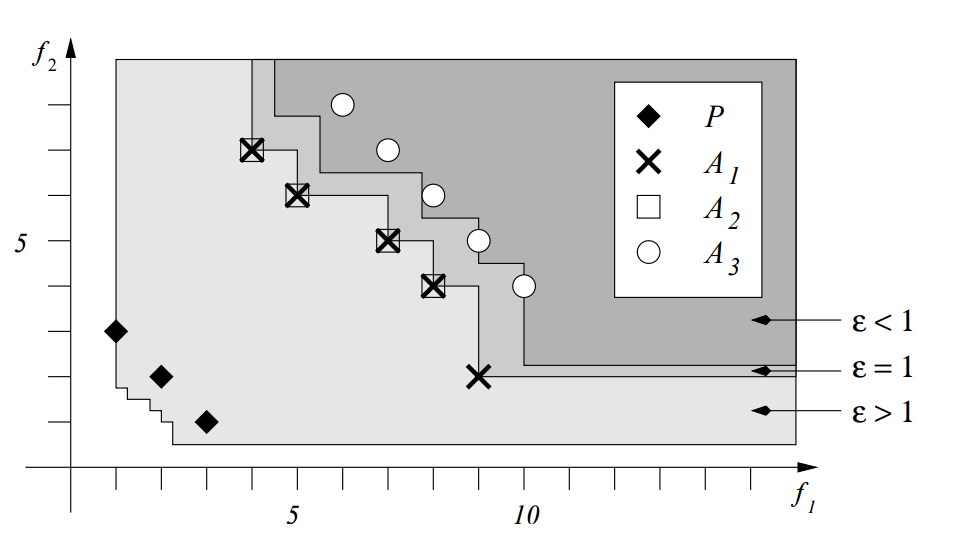
\includegraphics[width=.5\textwidth]{../images/BinaryEpsilonFigureLiftedFromZitzler}
\label{fig:binaryEpsilon}
\caption[Breakpoint values for the binary epsilon indicator $I_\epsilon$]{Any frontier $Z$ with solutions in the light gray area (closest to origin) would have $I_\epsilon (Z,A_1) > 1$; $I_\epsilon (A_1,A_1) = I_\epsilon (A_2,A_1) = 1$; any frontier $Z$ existing only in the darker gray areas such as $A_3$ would have $I_\epsilon (Z,A_1) < 1$}
\end{figure}

\paragraph{Unary hypervolume indicator $I_{H1}$ and binary hypervolume indicator $I_{H2}$}
For a frontier $Z$ comprised of solutions $\mathbf{z}=\braket{z^1,\ldots,z^N}$ and with the objective space defined such that the origin is the nadir point, then the volume of a single solution $\mathbf{z}_i$ is the volume of the hyperrectangle $r_i$ whose diagonal corners are the origin and the solution $\mathbf{z}_i$. The hypervolume of the frontier is the volume of the union of the hyperrectangles corresponding to the solutions in the frontier:
\begin{align}
I_{H1} (Z) = \text{vol} \left( \bigcup_{i = 1}^{|Z|} r_i \right)
\end{align}
Then define the binary hypervolume indicator of two frontiers $Z_1$ and $Z_2$ as \cite{zitzler1999evolutionary}
\begin{align}
I_{H2} (Z_1,Z_2) = I_{H1} (Z_1 + Z_2) - I_{H1} (Z_2)
\end{align}
where $I_{H1} (Z_1 + Z_2)$ is the unary hypervolume indicator of the merged frontier consisting of all solutions from frontiers $Z_1$ and $Z_2$. The binary hypervolume indicator provides the volume of frontier $Z_1$ that is not contained within frontier $Z_2$. Larger values of $I_{H1}$ correspond to frontiers occupying larger fractions of the objective space, indicating less conflict between the objectives. For frontiers $Z_1$ and $Z_2$ in comparable scales (that is, in normalized objective spaces), if $I_{H2}(Z_1, Z_2) > I_{H2}(Z_2, Z_1)$ this indicates less conflict between objectives in $Z_1$ than in $Z_2$. $I_{H2}$ can also be used to determine other dominance relationships between frontiers (see Tables \ref{tab:dominanceRelations} and \ref{tab:powerOfIndicatorTests}).


I developed a custom algorithm to solve for the unary hypervolume idicator. The details of the algorithm may be found in \S \ref{chap:appAHypervolumeAlgo}.

\begin{table}[]
\centering
\label{tab:dominanceRelations}
\resizebox{\textwidth}{!}{%
\begin{tabular}{|l|l|l|l|l|}
\hline
Relation           & \multicolumn{2}{c|}{Solutions}                                                                                                                                                                          & \multicolumn{2}{l|}{Frontiers}                                                                                                     \\ \hline
Strictly dominates & $\mathbf{z}^1 \succ \succ \mathbf{z}^2$ & $\mathbf{z}_i^1$ is better than $\mathbf{z}_i^2 \quad \forall 1 \le i \le N$                                                                                  & $Z_1 \succ \succ Z_2$ & $\exists \mathbf{z}^1 \in Z_1 \succ succ \mathbf{z}^2 \quad \forall \mathbf{z}^2 \in Z_2$                  \\ \hline
Dominates          & $\mathbf{z}^1 \succ \mathbf{z}^2$       & $\exists 1 \le i \le N : \mathbf{z}_i^1$ is better than $\mathbf{z}_i^2$, and $\mathbf{z}_i^1$ is not worse than $\mathbf{z}_i^2 \quad \forall 1 \le i \le N$ & $Z_1 \succ Z_2$       & every $\mathbf{z}^2 \in Z_2$ is dominated by at least one $\mathbf{z}^1 \in Z_1$                           \\ \hline
Better             &                                         &                                                                                                                                                               & $Z_1 \rhd Z_2$        & every $\mathbf{z}^2 \in Z_2$ is weakly dominated by at least one $\mathbf{z}^1 \in Z_1$ and $Z_1 \neq Z_2$ \\ \hline
Weakly dominates   & $\mathbf{z}^1 \succeq \mathbf{z}^2$     & $\mathbf{z}^1$ is at least as good as $\mathbf{z}^2$ in all objectives                                                                                        & $Z_1 \succeq Z_2$     & All solutions in $\mathbf{z}^2 \in Z_2$ are weakly dominated by a solution $\mathbf{z}^1 \in Z_1$          \\ \hline
Incomparable       & $\mathbf{z}^1 || \mathbf{z}^2$          & Neither $\mathbf{z}^1$ nor $\mathbf{z}^2$ weakly dominates the other                                                                                          & $Z_1 || Z_2$          & Neither $Z_1$ nor $Z_2$ weakly dominates the other                                                         \\ \hline
\end{tabular}%
}
\caption[Dominance relations between frontiers and solutions]{Definitions of dominance relations between solutions and frontiers \cite{zitzler2003performance}}
\end{table}

\begin{table}[]
\centering
\label{tab:powerOfIndicatorTests}
\resizebox{\textwidth}{!}{%
\begin{tabular}{|l|l|l|l|l|l|l|l|}
\hline
\multirow{2}{*}{} & \multicolumn{1}{c|}{\multirow{2}{*}{Name of indicator}} & \multicolumn{6}{c|}{Relation}                                                                                                                                                                                                                                                              \\ \cline{3-8} 
                  & \multicolumn{1}{c|}{}                                   & \multicolumn{1}{c|}{$\succ\succ$} & \multicolumn{1}{c|}{$\succ$} & \multicolumn{1}{c|}{$\rhd$}                             & \multicolumn{1}{c|}{$\succeq$}                & \multicolumn{1}{c|}{$=$}                              & \multicolumn{1}{c|}{$||$}                             \\ \hline
                  & $I_\epsilon$                                            & $I_\epsilon (Z_1,Z_2) < 1$        & -                            & $I_\epsilon (Z_1,Z_2)\le 1$ $I_\epsilon (Z_2,Z_1) > 1$ & $I_\epsilon (Z_1,Z_2)\le 1$                   & $I_\epsilon (Z_1,Z_2)= 1$ $I_\epsilon (Z_2,Z_1) = 1$ & $I_\epsilon (Z_1,Z_2)> 1$ $I_\epsilon (Z_2,Z_1) > 1$ \\ \hline
                  & $I_{H2}$                                                & -                                 & -                            & $I_{H2} (Z_1,Z_2)>0$ $I_{H2} (Z_2,Z_1) =0$             & $I_{H2} (Z_1,Z_2)\ge0$ $I_{H2} (Z_2,Z_1) =0$ & $I_{H2} (Z_1,Z_2)=0$ $I_{H2} (Z_2,Z_1) =0$           & $I_{H2} (Z_1,Z_2)>0$ $I_{H2} (Z_2,Z_1) >0$           \\ \hline
                  & $I_d$                                                   & -                                 & -                            & -                                                       & -                                             & -                                                     & -                                                     \\ \hline
                  & $I_s$                                                   & -                                 & -                            & -                                                       & -                                             & -                                                     & -                                                     \\ \hline
\end{tabular}%
}
\caption[Indicator comparisons to determine dominance relationships between frontiers]{Tests using indicators to determine dominance relationships between frontiers \cite{zitzler2003performance}. While general tests of dominance relationships may not be avaiable for some metrics (any cell with `-'), conclusions may still be drawn. For instance, $I_d(Z_1) < I_d(Z_2) \Rightarrow Z_2 \ntriangleright Z_1$.}
\end{table}

\paragraph{Unary distance indicator $I_d$} The unary distance indicator used for the analysis is analogous to the unary distance indicator described in \cite{czyzzak1998pareto}, but instead of computing the distance to a reference Pareto frontier I measure the average distance from the frontier to the ideal solution:
\begin{align}
I_d = \frac{\sum_{\mathbf{z} \in Z} ||\mathbf{z}^{\text{ideal}} - \mathbf{z} ||}{N}
\end{align}
Smaller values of $I_d$ correspond to frontiers that are closer to the ideal solution, which implies less conflict between the objectives.

\paragraph{Unary Spacing Indicator $I_s$} The unary spacing indicator, or Schott's spacing metric\cite{schott1995fault}, computes the standard deviation of the distance between points in the frontier, defined as
\begin{align}
I_s = \sqrt{\frac{1}{N-1} \sum_{\mathbf{z} \in Z} (d_z - \overbar{d})^2}
\end{align}
where
\begin{align}
d_z = \min_{\mathbf{y} \in Z, \mathbf{y} \neq \mathbf{z}} ||\mathbf{z} - \mathbf{y}||
\end{align}
and $\overbar{d}$ is the average of all $d_z$. In EMO, the spacing indicator provides a measure of an algorithm's ability to search the frontier space uniformly. Here, the spacing metric provides a measure of the flexibility afforded to the decision maker under each climate scenario. Larger spacing metrics imply larger sacrifices between decisions and less flexibility.

\subsubsection{Quantifying conflict between objectives within a frontier}

The above methods provide frontier-level metrics of conflict and tradeoffs. To determine the degree of conflict between two objectives within a single frontier, we employ an approach used in many-objective optimization. Given the increased difficulty in solving many-objective optimization problems \cite{khare2003performance}, researchers in this field seek to reduce the number of objectives considered in the model. To determine which objectives most strongly influence the shape of the frontier, they compute the correlation between each pair of objectives \cite{deb2005finding}. The objective pairs with the most negative correlation are most in conflict. To rank the relative conflict between objectives in each climate scenario, I compute their Pearson correlation coefficients:
\begin{align}
\rho_{X,Y} = \frac{\text{cov}(X,Y)}{\sigma(X)\sigma(Y)}
\end{align}
where, for objectives $x$ and $y$, $X$ and $Y$ are
\begin{align}
X = \{ \mathbf{z}_x^1, \mathbf{z}_x^2, \ldots, \mathbf{z}_x^{|Z|} \} \\
Y = \{ \mathbf{z}_y^1, \mathbf{z}_y^2, \ldots, \mathbf{z}_y^{|Z|} \}
\end{align}